% TODO: venue template. No .cls or .sty was present in the repository, so this is a
% generic two-column article sized to the 4-page limit (excluding references).
% Swap \documentclass and the geometry block for the venue's style file when it
% arrives; nothing below depends on them.
\documentclass[10pt,twocolumn]{article}
\usepackage[margin=0.75in]{geometry}
\usepackage{booktabs,graphicx,amsmath,amssymb,microtype}
\usepackage[hidelinks]{hyperref}
\usepackage[font=small,skip=3pt]{caption}
\setlength{\abovedisplayskip}{4pt}
\setlength{\belowdisplayskip}{4pt}

\title{\vspace{-1.2em}Gaussian context sampling for imbalanced regression\\
       with tabular in-context learners}
\author{TODO: authors, affiliation}
\date{}

\begin{document}
\maketitle

\begin{abstract}
% TODO: write last, from paper/RESULTS_SUMMARY.md. One sentence each:
% (i) tabular in-context learners draw their context uniformly;
% (ii) we re-weight that context by a Gaussian over the target;
% (iii) what it does -- state the trade-off, not only the wins;
% (iv) the scope it holds in.
\end{abstract}

\section{Introduction}
% ~0.6 page.
% - Imbalanced regression: rare target regions are predicted poorly, and the usual
%   remedies (LDS/FDS, RankSim, ConR) re-weight the LOSS during training.
% - Tabular in-context learners (TabPFN-2.5, TabICL) make a prediction by
%   conditioning on a context set rather than by fitting weights, which exposes a
%   lever none of those methods have: WHICH rows enter the context.
% - That context is normally sampled uniformly. Nothing requires it to be.
% - Contributions:
%   (1) a Gaussian context-sampling scheme with a centre and width redrawn per
%       episode;
%   (2) applied at two levels -- per-dataset fine-tuning, and continued
%       pre-training on the model's own synthetic prior, which is dataset
%       independent;
%   (3) an encoder trained end-to-end through a frozen in-context model, for ECG
%       age regression;
%   (4) a controlled evaluation: every arm is matched against a uniform control
%       with identical cost, and against an inverse-density context baseline.

\section{Method}
% ~0.7 page.
\subsection{Context and query sampling}
% - Define context vs query. Queries are drawn FIRST and left unweighted, so the
%   evaluation distribution is unchanged by the intervention.
Each episode draws a centre and a width,
\begin{equation}
\mu = Q_y(u),\quad u \sim U(0.05, 0.95), \qquad
\sigma = \mathrm{sd}(y)\, e^{v},\quad v \sim U(\log 0.15, \log 1.5),
\end{equation}
and weights each candidate context row by
$w_i \propto \exp\!\big(-\tfrac12((y_i-\mu)/\sigma)^2\big)$.
% - Selection is Gumbel-top-$k$ in log space: the Gaussian weights underflow to
%   exactly zero several sigma out, which is precisely the regime of interest.
% - Redrawing $(\mu,\sigma)$ every episode means the model sees a FAMILY of skews
%   rather than one fixed one.

\subsection{Two regimes}
% - Per-dataset fine-tuning: the context is Gaussian-sampled while fine-tuning on
%   the target dataset.
% - Prior-level continued pre-training: TabICL is given 3000 further steps on its
%   OWN synthetic prior, with rows reordered so the positional context/query cut
%   falls on a target-concentrated context. The resulting model has never seen any
%   evaluation dataset. TabPFN-2.5 cannot be tested this way -- the checkpoint
%   ships, the prior generator does not.
% - Controls: `uniform' performs a permutation of identical shape and cost, and
%   `target-balanced' samples with probability inverse to target-bin frequency.

\subsection{ECG encoder}
% - A ResNet1d-Wang is trained so that a FROZEN in-context model predicts age well
%   from its features; gradients reach the encoder through the frozen body.
% - E1 supervised L1; E2 through TabPFN; E3 through stock TabICL; E4 through
%   Gaussian-prior TabICL. All share one warm start, so differences isolate the body.

\section{Experiments}
% ~2.3 pages.
\subsection{Setup}
% - Datasets: Abalone, Communities and Crime, Wine Quality White, PTB-XL age.
% - Shot regions follow Yang et al. (2021): many >100, few <20 training rows per bin.
% - PTB-XL age bands: <30, 30--60, >=60. Five seeds everywhere; mean +- sd reported.
% - PTB-XL uses the OFFICIAL partition. State plainly why: the balanced-resample
%   protocol draws its test set from all records, and every encoder here was fitted
%   on the official train split, so ~80\% of that test set is data the encoder has
%   already seen. See the limitations paragraph.

\begin{table}[t]\centering\small
\caption{TabICL, synthetic-prior continued pre-training only. No model has seen any
evaluation dataset. Mean $\pm$ sd over 5 seeds; lower is better.}
\label{tab:1a}
\begin{tabular}{lccccc}
\toprule
& Many & Medium & Few & Overall & GM \\
\midrule
\multicolumn{6}{l}{\textit{Abalone}} \\
zero-shot & 1.146\,$\pm$\,0.081 & 2.595\,$\pm$\,0.031 & 6.219\,$\pm$\,0.030 & 2.956\,$\pm$\,0.038 & 1.649\,$\pm$\,0.085 \\
uniform context & 1.148\,$\pm$\,0.082 & \textbf{2.578\,$\pm$\,0.031} & \textbf{6.189\,$\pm$\,0.031} & \textbf{2.943\,$\pm$\,0.039} & \textbf{1.645\,$\pm$\,0.077} \\
target-balanced context & \textit{TODO} & \textit{TODO} & \textit{TODO} & \textit{TODO} & \textit{TODO} \\
Gaussian context & \textbf{1.128\,$\pm$\,0.087} & 2.618\,$\pm$\,0.024 & 6.385\,$\pm$\,0.037 & 3.000\,$\pm$\,0.028 & 1.665\,$\pm$\,0.075 \\
\midrule
\multicolumn{6}{l}{\textit{Communities}} \\
zero-shot & 0.0587\,$\pm$\,0.0013 & \textbf{0.1680\,$\pm$\,0.0054} & 0.2552\,$\pm$\,0.0083 & 0.1598\,$\pm$\,0.0040 & 0.0898\,$\pm$\,0.0068 \\
uniform context & 0.0585\,$\pm$\,0.0014 & 0.1683\,$\pm$\,0.0055 & \textbf{0.2549\,$\pm$\,0.0082} & \textbf{0.1598\,$\pm$\,0.0040} & \textbf{0.0896\,$\pm$\,0.0072} \\
target-balanced context & \textit{TODO} & \textit{TODO} & \textit{TODO} & \textit{TODO} & \textit{TODO} \\
Gaussian context & \textbf{0.0577\,$\pm$\,0.0015} & 0.1737\,$\pm$\,0.0066 & 0.2854\,$\pm$\,0.0037 & 0.1708\,$\pm$\,0.0031 & 0.0937\,$\pm$\,0.0042 \\
\midrule
\multicolumn{6}{l}{\textit{Wine Quality White}} \\
zero-shot & \textbf{0.335\,$\pm$\,0.008} & \textbf{1.195\,$\pm$\,0.060} & \textbf{2.453\,$\pm$\,0.024} & \textbf{0.785\,$\pm$\,0.020} & \textbf{0.256\,$\pm$\,0.008} \\
uniform context & 0.337\,$\pm$\,0.009 & 1.199\,$\pm$\,0.059 & 2.456\,$\pm$\,0.025 & 0.787\,$\pm$\,0.019 & 0.267\,$\pm$\,0.009 \\
target-balanced context & \textit{TODO} & \textit{TODO} & \textit{TODO} & \textit{TODO} & \textit{TODO} \\
Gaussian context & 0.349\,$\pm$\,0.011 & 1.280\,$\pm$\,0.051 & 2.517\,$\pm$\,0.022 & 0.828\,$\pm$\,0.018 & 0.353\,$\pm$\,0.010 \\
\bottomrule
\end{tabular}

\end{table}

\begin{table}[t]\centering\small
\caption{TabPFN-2.5, per-dataset fine-tuning. Learning rate selected on validation.}
\label{tab:1b}
\begin{tabular}{lcccc}
\toprule
& Many & Medium & Few & Overall \\
\midrule
\multicolumn{5}{l}{\textit{Abalone}} \\
zero-shot & \textit{TODO} & \textit{TODO} & \textit{TODO} & \textit{TODO} \\
uniform fine-tuning & \textbf{1.208\,$\pm$\,0.086} & 2.357\,$\pm$\,0.105 & 5.767\,$\pm$\,0.217 & 2.786\,$\pm$\,0.108 \\
Gaussian fine-tuning & 1.584\,$\pm$\,0.145 & \textbf{1.392\,$\pm$\,0.094} & \textbf{4.127\,$\pm$\,0.151} & \textbf{2.202\,$\pm$\,0.062} \\
\midrule
\multicolumn{5}{l}{\textit{Communities}} \\
zero-shot & \textbf{0.0592\,$\pm$\,0.0015} & 0.1677\,$\pm$\,0.0049 & 0.2577\,$\pm$\,0.0053 & 0.1606\,$\pm$\,0.0035 \\
uniform fine-tuning & 0.0597\,$\pm$\,0.0016 & 0.1678\,$\pm$\,0.0051 & 0.2538\,$\pm$\,0.0062 & 0.1596\,$\pm$\,0.0026 \\
Gaussian fine-tuning & 0.0646\,$\pm$\,0.0031 & \textbf{0.1617\,$\pm$\,0.0042} & \textbf{0.2348\,$\pm$\,0.0012} & \textbf{0.1530\,$\pm$\,0.0020} \\
\midrule
\multicolumn{5}{l}{\textit{Wine Quality White}} \\
zero-shot & 0.427\,$\pm$\,0.013 & 1.432\,$\pm$\,0.022 & 2.455\,$\pm$\,0.027 & 0.926\,$\pm$\,0.011 \\
uniform fine-tuning & \textbf{0.370\,$\pm$\,0.019} & 1.295\,$\pm$\,0.023 & 2.375\,$\pm$\,0.025 & 0.837\,$\pm$\,0.011 \\
Gaussian fine-tuning & 0.391\,$\pm$\,0.038 & \textbf{1.138\,$\pm$\,0.055} & \textbf{2.250\,$\pm$\,0.104} & \textbf{0.783\,$\pm$\,0.031} \\
\bottomrule
\end{tabular}

\end{table}

\begin{table*}[t]\centering\small
\caption{PTB-XL age prediction, mean absolute error in years, on the official test
split. Band-macro is the unweighted mean of the three band errors.}
\label{tab:2}
\begin{tabular}{lcccccc}
\toprule
& $<$30 & 30--60 & $\geq$60 & Natural & Band-macro & GM \\
\midrule
ResNet (vanilla) & 9.456\,$\pm$\,0.000 & \textbf{6.294\,$\pm$\,0.000} & 8.940\,$\pm$\,0.000 & 7.548\,$\pm$\,0.000 & 8.230\,$\pm$\,0.000 & 4.904\,$\pm$\,0.000 \\
ResNet + RankSim + ConR & \textit{TODO} & \textit{TODO} & \textit{TODO} & \textit{TODO} & \textit{TODO} & \textit{TODO} \\
E2 + stock TabPFN-2.5 & \textbf{7.657\,$\pm$\,0.009} & 7.245\,$\pm$\,0.006 & \textbf{7.628\,$\pm$\,0.011} & \textbf{7.421\,$\pm$\,0.003} & \textbf{7.510\,$\pm$\,0.005} & \textbf{4.724\,$\pm$\,0.023} \\
E2 + Gaussian TabPFN-2.5 & 7.657\,$\pm$\,0.009 & 7.245\,$\pm$\,0.006 & 7.628\,$\pm$\,0.011 & 7.421\,$\pm$\,0.003 & 7.510\,$\pm$\,0.005 & 4.724\,$\pm$\,0.023 \\
E3 + stock TabICL & \textit{TODO} & \textit{TODO} & \textit{TODO} & \textit{TODO} & \textit{TODO} & \textit{TODO} \\
E3 + Gaussian TabICL & \textit{TODO} & \textit{TODO} & \textit{TODO} & \textit{TODO} & \textit{TODO} & \textit{TODO} \\
\bottomrule
\end{tabular}

\end{table*}

\begin{table}[t]\centering\small
\caption{Encoder training against prediction head. The gap between the two column
groups is the contamination in the balanced protocol, not a property of the method.}
\label{tab:3}
\begin{tabular}{lcccc}
\toprule
& \multicolumn{2}{c}{Natural (official split)} & \multicolumn{2}{c}{Balanced (DIR split)} \\
\cmidrule(lr){2-3}\cmidrule(lr){4-5}
Encoder & stock head & Gaussian head & stock head & Gaussian head \\
\midrule
E1 (supervised L1) & 7.428\,$\pm$\,0.008 & 7.654\,$\pm$\,0.041 & 7.330\,$\pm$\,0.067 & 7.162\,$\pm$\,0.070 \\
E2 (through TabPFN) & 7.428\,$\pm$\,0.004 & 7.648\,$\pm$\,0.015 & 7.258\,$\pm$\,0.090 & 7.108\,$\pm$\,0.080 \\
E3 (through stock TabICL) & \textbf{7.353\,$\pm$\,0.002} & \textbf{7.585\,$\pm$\,0.017} & \textbf{7.152\,$\pm$\,0.090} & \textbf{7.042\,$\pm$\,0.120} \\
E4 (through Gaussian TabICL) & 7.469\,$\pm$\,0.004 & 7.617\,$\pm$\,0.007 & 7.384\,$\pm$\,0.080 & 7.392\,$\pm$\,0.108 \\
\bottomrule
\end{tabular}

\end{table}

\begin{figure}[t]\centering
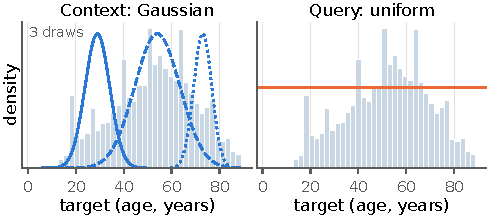
\includegraphics[width=\columnwidth]{figs/fig1_method.pdf}
\caption{Context rows are weighted by a Gaussian over the target, with centre and
width redrawn each episode; queries stay uniform.}
\label{fig:1}
\end{figure}

\begin{figure}[t]\centering
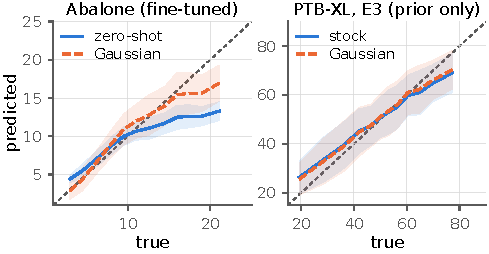
\includegraphics[width=\columnwidth]{figs/fig2_pred_vs_true.pdf}
\caption{Binned predictions against truth, $\pm1$ sd. TODO: state in the caption
which arms and whether predictions are seed-averaged.}
\label{fig:2}
\end{figure}

\subsection{Results}
% - Table~\ref{tab:1a}: prior-level arms against their matched uniform control.
% - Table~\ref{tab:1b}: per-dataset fine-tuning.
% - Table~\ref{tab:2}: PTB-XL, against the ResNet baselines.
% - Table~\ref{tab:3}: encoder x head.
% - Significance: paired bootstrap CIs and per-seed win counts from
%   imbreg/results/metrics/significance.csv. Quote intervals, not just means.

\subsection{The trade-off}
% REQUIRED paragraph -- do not soften it. Gaussian context sampling moves error
% rather than removing it: the frequent region and the 30--60 band get WORSE in
% every configuration measured. Report the sign and size of that loss next to every
% gain, and say under which evaluation weighting the net is positive.

\section{Conclusion and limitations}
% ~0.2 page.
% - What holds, and in what scope.
% - Limitations to state explicitly:
%   (i) the prior-level result does not transfer to the tabular benchmarks;
%   (ii) the balanced protocol re-uses encoder training data, so Table~\ref{tab:3}'s
%        balanced columns are optimistic;
%   (iii) the encoders stopped improving after a few hundred steps, so they are not
%        converged;
%   (iv) single ECG dataset; no claim beyond it.

\bibliographystyle{plain}
% TODO: references -- Yang et al. 2021 (DIR), Hollmann et al. (TabPFN),
% TabICL, Ribeiro & Moniz 2020 (SERA), RankSim, ConR.
\end{document}
